%----------------------------------------------------------------------------------------
%	RESULTS
%----------------------------------------------------------------------------------------
% TODO divide into subsections: Results for Agent, Results for Experiment, Comparison
% TODO make a 3x2 grid with different risks.

\large{Solving the risk sensitive POMDP}

\normalsize

State space must be augmented two times:
\begin{figure}
\begin {center}
\begin {tikzpicture}[-latex ,auto ,node distance =6cm and 6cm ,on grid ,
semithick ,
state/.style ={ circle ,fill=black!20, minimum width =3 cm}]
\node[state] (A) [align=center] {Observation\\Time};
\node[state] (B) [right of=A,align=center] {Belief\\Time};
\node[state] (C) [right of=B,align=center] {Belief\\Wealth};


\path (A) edge [line width=2mm, align=center] node[left] {bayes} (B);
\path (B) edge [bend left = -25,line width=2mm,align=center] node[below =0.25 cm] {sell\\$1.0$} (C);
\end{tikzpicture}
\end{center}
\end{figure}


Observation and time to belief and time
belief and time to belief and wealth

\cite{marecki} showed that in belief time space POMDPs can be solved for arbitrary utility functions using \textbf{reverse value iteration}.

\begin{figure}
    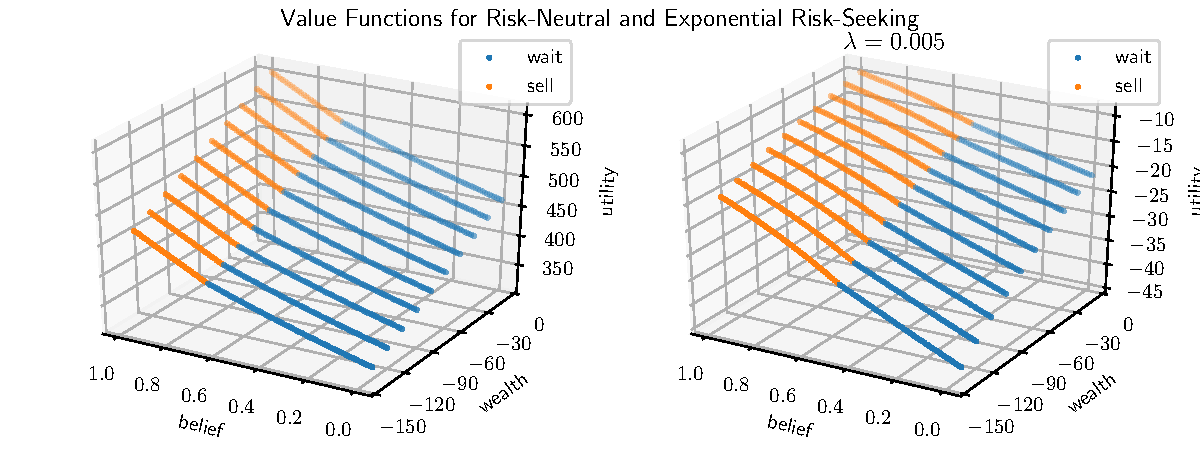
\includegraphics[width=0.9\linewidth]{img/exp_policy.pdf}\\
    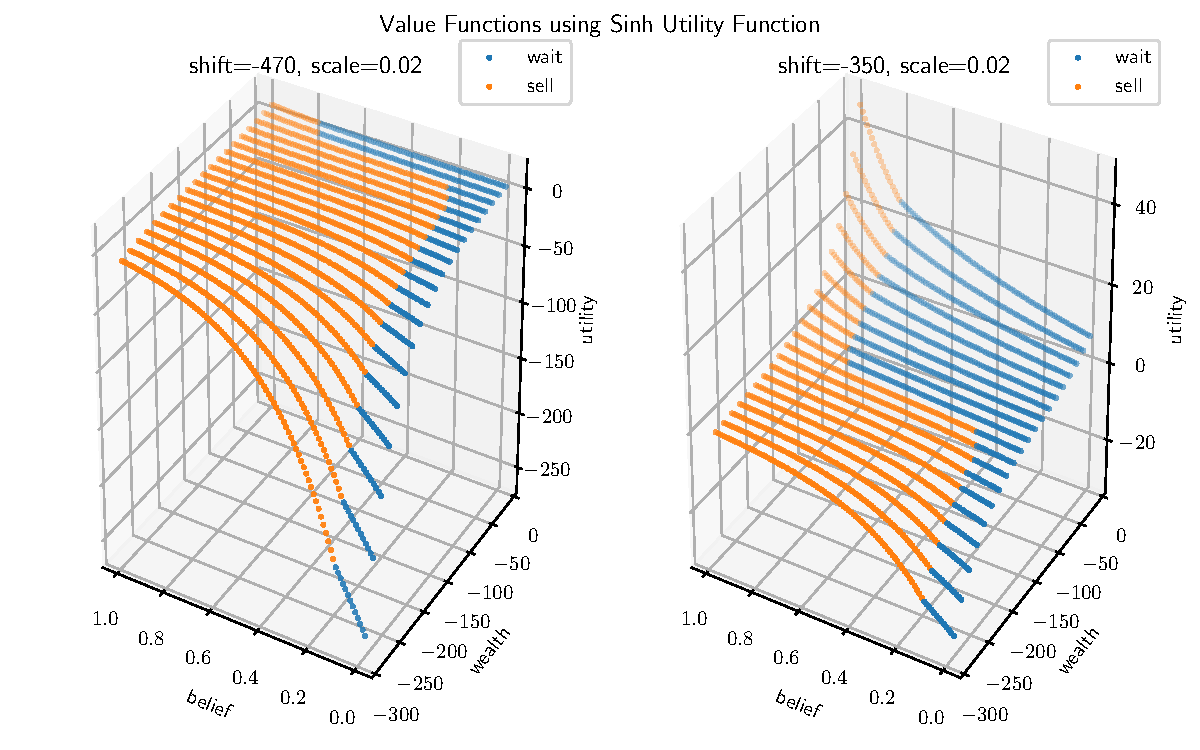
\includegraphics[width=0.9\linewidth]{img/sinh_policy.pdf}\\
    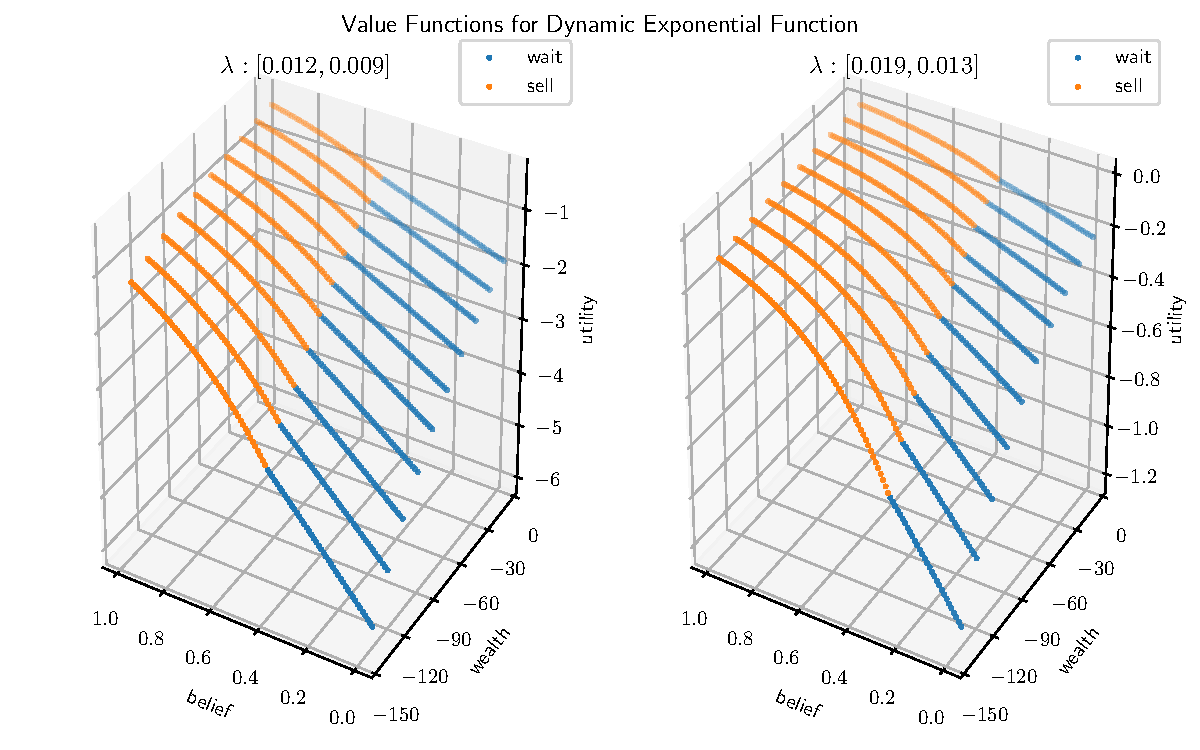
\includegraphics[width=0.9\linewidth]{img/dyn_policy.pdf}
    \caption{Value functions exhibiting different risk-behaviors; from top left: risk neutral agent (utility function is the identity function), risk-seeking agent with exponential utility function, two fixed time agents with different time thresholds, two agents with dynamic exponential utility function in the expensive expert scenario.}
\end{figure}

\textbf{The original problem:}
\begin{itemize}
\item[①] Choose utility function with risk parameter.
\item[②] Perform value iteration.
\item[③] Derive policy.
\end{itemize}

\textbf{The inverse problem:}
\begin{itemize}
\item[①] Observe behavior.
\item[②] Estimate policy.
\item[③] Derive utility function and risk parameters.
\end{itemize}

The original problem is easy to solve, unfortunately for the inverse problem no solution is known. $\rightarrow$ Perform grid-search and choose optimal utility function.
